\documentclass[conference]{IEEEtran}
\usepackage{algorithm2e}
\usepackage{graphicx}
\usepackage{subfigure}
\usepackage{multirow}
\usepackage{booktabs}
\usepackage{url}
\usepackage{listings}
\lstset{basicstyle=\scriptsize\ttfamily, keywordstyle=\bfseries}

\begin{document}
\title{Original Method: \\
    Smithers: Wake Word Exploration for Resource-Constrained Devices}
\author{ Jacob Jones \\
    ECE 551, Problems \\
    The University of New Mexico \\
    Albuquerque, NM 87131, USA \\
    jacobearljones@unm.edu}

\maketitle

\begin{abstract}

    Many consumer electronic devices contain digital "smart assistants"
    that listen and respond to voice commands.
    Many of the devices that run these assistants are constrained memory and battery limitations
    and are not capable running word recognition models at all times.
    These devices rely on trigger words, or "wake words", as the first step
    in the word recognition pipeline.
    This project will explore wake words with a focus on their application
    on devices with limited computational resources.

\end{abstract}
\begin{IEEEkeywords}
    machine learning; convolutional neural nets; wake words; speech recognition; embedded computing
\end{IEEEkeywords}
\IEEEpeerreviewmaketitle

\section{Background}

\subsection{Motivation}

Digital "smart" assistants such as Alexa, Siri, and Google Assistant are commonly found
in smartphones, smart watches, and smart speakers.
A common fear is that these devices are always spying on us, listening to everything we say.
These devices are indeed always listening,
but more often than not,
these devices only care about a few key words.

Many of these devices do not have the resources to interpret an entire dictionary.
For low-power edge devices such as smart watches and smart speakers,
full-dictionary word recognition is too computationally costly.
Resource constrains, such as memory and battery limitations,
restrict the capabilities of the always-on word recognition models. 
Typically, these devices are trained to recognize only a select few words -
"Hey Alexa", "Hey Siri", and "Hey Google", for the big three smart assistants.
These "wake words" activate the assistant 
and the commands that follow are either processed by a more advanced model
or are sent to the cloud for further processing.

My technical interests lie where hardware and software intersect.
Embedded devices with specifically-designed hardware and software
fit perfectly within this niche.
Many embedded devices are resource-constrained and must make sacrifices
to optimize the limited available power and computational resources.
I have bought into the Google Home ecosystem and the Google Assistant 
has proven to be incredibly handy around the home.
It naturally follows that I am interested in researching these smart home devices
and the wake words processes that they implement.

Every smart assistant needs a wake word that's both memorable and relatively uncommon.
Siri (Apple), Alexa (Amazon), Bixby (Samsung), and Cortana (Microsoft)
are all given names to personify the smart assistant.
For this project, I will be developing the beginnings of a new digital assistant
in the form of wake word recognition.
My smart assistant will be named "Smithers".
Smithers is the faithful assistant to the curmudgeonly Mr. Burns 
in one of my favorite television shows, the Simpsons.
I believe this is an excellent (and fun to say) name for a digital assistant.

\begin{figure}[htbp]
    \centerline{
\includegraphics[width=0.35\textwidth]{figs/smithers.jpg}}
    \caption{Smithers (right) and Mr. Burns (left)}
    \label{fig:1}
\end{figure}

\subsection{Expected Contribution}
The goal of this project is to create a machine learning model capable of wake word recognition.
This model could be used as a jumping-off point for exploring wake word recognition
or serve as a foundation for more advanced projects
This project explains key concepts in wake word recognition
and explores fundamental components such as mel-frequency cepstral coefficients and convolutional neural nets.
This project also explores how preexisting models handle wake word recognition,
comparing methods and processes and drawing inspiration from these ideas.

\subsection{Competing Methods}
Three of the big tech companies - Amazon, Apple, and Google - 
develop competing smart assistants.
All three of these companies have produced papers concerning speech recognition.
All three of these companies smart assistants utilize convolutional neural nets (CNNs)
and all three of these smart assistants process the audio with a mel filterbank.
Fundamental concepts from these papers will be applied to this project.

In \textit{Small-footprint Keyword Spotting Using Deep Neural Nets},
researchers at Google discuss a computationally cost-effective neural net used to detect key words.
This paper does not directly discuss wake word detection
but describes the methods use to process incoming audio.
The features used in this CNN are mel filterbank energies of the audio signal.
These researchers achieved the best results
by applying RelU activation functions for the CNN layers \cite{smallfoot}.

In \textit{Accurate Detection of Wake Word Start and End Using a CNN}, 
Amazon researchers also suggest using mel filterbank to process the incoming audio
for a non-linear frequency response similar to how humans perceive sound \cite{wordstart}.
The Amazon CNN is a two-part model that both detects wake words
and detects the start point and end points of these words.

Perhaps the research most relevant to this project come from Apple engineers working on Siri.
The focus on \textit{Efficient Voice Trigger Detection for Low Resource Hardware}
is on CNNs running on embedded hardware and aligns well with the goals of this project \cite{Efficient}.
These researchers suggest quantizing 32-bit floating-point numbers 
within the mel filterbank energy calculations to 8-bit fixed-point integers. 
Fixed-point math is less computationally-intensive than floating-point math
and these Apple researchers determined the decrease in accuracy is a worthy tradeoff
for an increase in performance.
These researchers also suggest using sigmoid activation 
to bound weights between $[0,1]$ for more efficient math on the rounded fixed-point numbers.

\subsection{Comparisons with Competing Methods}

As with Alexa, Siri, and Google Assistant, Smithers makes predictions
using a convolutional neural net trained on mel frequency energies.
Smithers, however, is a much simpler model.
More technical details will be revealed in Section \ref{sec:method}, \textit{Method}.

Smithers is a binary classifier - either it detected "Hey Smithers" or it didn't.
This is the same route Amazon took with their Alexa CNN \cite{wordstart}.
The Google Assistant and Siri models are both multiclass classifiers that
detect the individual phonemes that make up the incoming words \cite{smallfoot}\cite{Efficient}.
A prediction is made from the combined probabilities of the individual phonemes.

Smithers, Alexa, Siri, and Google Assistant all calculate the mel frequency energies
by framing the audio into 25ms frames.
The frames in Smithers do not overlap, resulting in 40 frames per second.
The frames in Alexa, Siri, and Google Assistant both overlap at a rate of 100 frames per second.
For each frame, Smithers calculates 13 mel frequency energies, Alexa calculates 64 mel frequency energies, 
Siri calculates 13 mel frequency energies, and Google Assistant calculates 40 mel frequency energies.
Smithers makes predictions on a window of 40 consecutive frames. 
Siri predicts on 19 consecutive frames while Google Assistant predicts on 40 consecutive frames.

\section{Method} \label{sec:method}

Smithers is a wake word detector that listens for the phrase "Hey Smithers"
Smithers detects wake word through inference by a convolutional neural net (CNN).
Like all CNN's, Smithers requires a well-constructed data set
with quantifiable and properly-labeled features.
This section details the methodology and processes
behind the Smithers CNN training and implementation.
Figure \ref{fig:flow} shows an flowchart of these processes.

\begin{figure}[htbp]
    \centerline{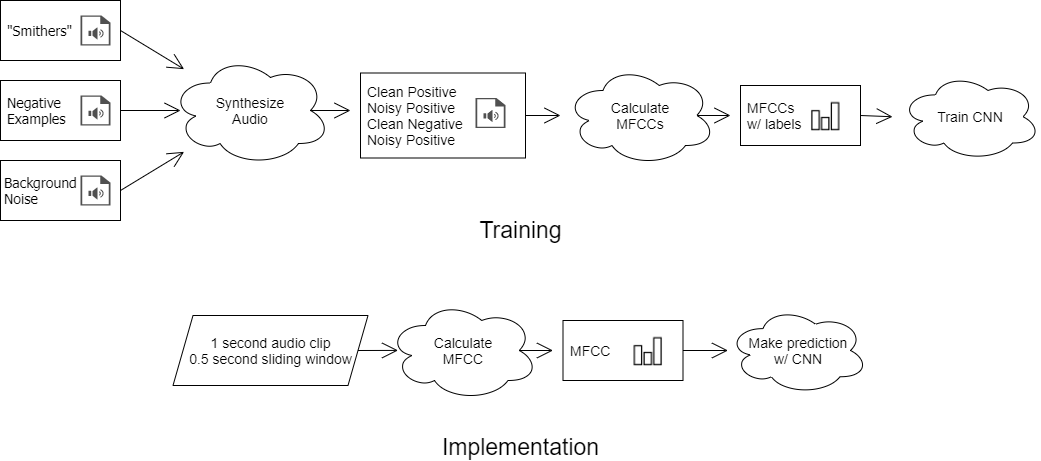
\includegraphics[width=0.5\textwidth]{figs/flow.png}}
    \caption{Project Flowchart}
    \label{fig:flow}
\end{figure}

\subsection{Wake word selection}
As noted earlier, the wake word was chosen
as an allusion to a personal assistant in the television show "The Simpsons".
The first iteration of this project used the wake word "Smithers".
In independent testing, this first iteration exhibited a high rate of false positives. 
This model triggered off the sounds "smith" and "ers",
sounds commonly uttered in everyday conversation.
For wake word detectors, Tsai et. al. suggest using a wake word
with at least three syllables \cite{syllables}. 
Switching the wake words from "Smithers" to "Hey Smithers"
greatly decreased the number of false positives.
Increasing the number of phonemes, or distinguishable sounds, greatly helped the model 
correctly recognize the wake word phrase.

\subsection{Code}
Smithers is built in Python and uses TensorFlow and Keras as the machine learning frameworks.
Smithers also uses the python\_speech\_features library for feature extraction
and TensorFlow Lite for model packaging and deployment.
Several selected code excerpts can be found in the Appendix.

Portions of the code were adapted from Shawn Hymel's \textit{TensorFlow Lite Speech Recognition Demo}
and Chengwei Zhang's instructional GitHub repository \cite{hymel} \cite{tony}.

\subsection{Dataset} \label{sec:dataset}
The Smithers dataset was synthesized rather than naturally recorded.
This is because it is much quicker to artificially create a large set of audio clips
rather than collect them manually.
The ingredients for this synthesized dataset were 
36 manually-recorded positive examples of the wake words "hey Smithers",
130 manually-recorded negative examples from randomly chosen words,
130 negative examples drawn from the Google Speech Commands dataset,
and 200 samples of background noise drawn from the Harvard ESC-50 dataset.

The positive examples were recorded by repeating the wake phrase "Hey Smithers"
in different inflections and speaking volume
and cutting the examples into individual tracks.
The manually-recorded negative examples were recorded 
by reading words from a online random paragraph generator
and again cutting the words into individual tracks.
The Google Speech Commands dataset contains common words such as "stop", "left", and "seven" \cite{aiblog}.
The ESC-50 dataset contains background noise field recordings
from sources such as wind, rain, and running water \cite{noise}.

To synthesize the dataset, a simple routine was constructed. The pseudocode is as follows: 
\begin{enumerate}
    \item Randomly choose one positive example, one negative example, and one background noise recording
    \item From the background noise recording, select a random 1-second interval
    \item Choose a random starting point within a one-second interval
    \item Overlay the positive example onto the noise interval at the random start point and save
    \item Overlay the negative example onto the noise interval at the random start point and save
    \item Overlay the positive example onto one-second of silence at the random start point and save
    \item Overlay the negative example onto one-second of silence at the random start point and save
\end{enumerate}
This routine is repeated 5,000 times. 
This processes creates 5,000 positive noise-free examples,
5,000 positive noisy examples,
5,000 negative noise-free examples,
and 5,000 negative noisy examples, building a 20,000 examples dataset.
These examples are all exactly one-second long
and the command samples all start at a random point within the one-second window.
This one-second long window was chosen primarily for convenience.
Appendix \ref{appendix:synthesis} shows the code for this routine.

The selected categories of noise field recordings - running water, wind, and rain - 
were chosen because of their similarity to both 
environmental noise indicative of the real world and high-frequency white noise.
I believe that introducing these noise sources will help model to learn to reject
both common household noise and other common high-frequency noise sources,
such as electrical noise.

The mel-frequency cepstral coefficients are then calculated for each example in the dataset.
In addition, labels are assigned for each example - 
$1$ for the positive examples and $0$ for the negative examples.
Section \ref{sec:mfcc}, \textit{Mel-frequency cepstral coefficients},
discusses these features and their extraction.

After the features are extracted, the dataset is shuffled 
and split into a training set, a validation set, and a test set at a ratio of 80:10:10. 
That is, the training set consists of 16,000 examples and the validation and test sets 
each consist of 2,000 examples.
These sets are then used for the CNN training, validation, and evaluation.


\subsection{Mel-frequency cepstral coefficients} \label{sec:mfcc}
The features that the Smithers model trains and infers upon 
are an audio signal's mel-frequency cepstral coefficients (MFCCs).
These MFCCs are set of metrics that describe a non-linear transformation of the signal's Fourier transform.
MFCCs were chosen as the model's trainable feature because of their accurate representation
of a word's individual phonemes \cite{lyons}.
Whereas a raw spectrogram shows the amplitudes of every one of signal's constituent frequencies,
the MFCCs represent the amplitudes of particular frequencies after a series of filters and transformations.
This process distills an audio signal into a minimal set of representative data relevant for distinguishing phonemes, 
effectively highlighting what's important and stripping away what's not.

To calculate the MFCCs, a signal is first windowed into short segments
and the Fast Fourier transforms (FFTs) are taken on each window.
For each window, the transform is filtered by a mel filterbank,
the logs of power of the mel frequencies are calculated,
and the discrete cosine transform of the logs are then taken.
The MFCCs are the resulting amplitudes of the transformed mel frequencies for each window.
This process is automated by the \textit{python\_speech\_features} Python library.

Figure \ref{fig:filterbank} shows the mel filterbank \cite{lyons}.
The key idea behind this filterbank is that the human ear does not have a linear frequency response.
Humans are better at perceiving differences between lower frequencies
than differences between higher frequencies.
The mel filterbank emphasizes this logarithmic-like response and helps a model "hear" as a human would hear.

\begin{figure}[htbp]
    \centerline{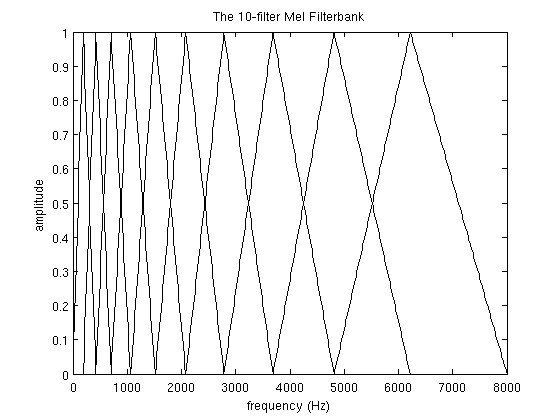
\includegraphics[width=0.5\textwidth]{figs/filterbank.png}}
    \caption{Mel filterbank \cite{lyons}}
    \label{fig:filterbank}
\end{figure}

The MFCC process calculates 40 different coefficients,
with the coefficient number increasing with it representative frequency.
Coefficients above number 13 are not typically used in speech recognition models,
such as in Apple's digital assistant Siri,
because humans typically do not have the ability 
to speak or hear at these high frequencies (roughly above 16kHz) \cite{Efficient}.
The Smithers model follows suit and uses the first 13 MFC coefficients as the trainable features.

For the Smithers model, the audio clips were first downsampled to a 10kHz bit rate.
The MFCCs were then calculated using the \textit{mfcc} function 
in the \textit{python\_speech\_features} library.
This function accepts a number of input parameters including the window size and number of coefficients.
For Smithers, the audio clips were segmented into 25ms frames and the first 13 coefficients were calculated.
One-second audio clips divide into 40 25ms frames and the resulting calculations create a 13x40 array for each clip.
Following in the footsteps of Apple,
these MFCCs are then casted from 64-bit floating point numbers 
to 8-bit signed integers to reduce the model size \cite{Efficient}.
This is especially important for models running on resource-constrained hardware.

One benefit of the MFCC process is that each audio example is essentially transformed into a 13x40 pixel image.
Convolutional neural nets excel at this sort of image recognition problem. 
Figure \ref{fig:pos} shows a visualization of a positive example 
and Figure \ref{fig:neg} show a visualization of a negative example.
Appendix \ref{appendix:mfcc} shows the code used to calculate the MFCCs.


\begin{figure}[htbp]
    \centerline{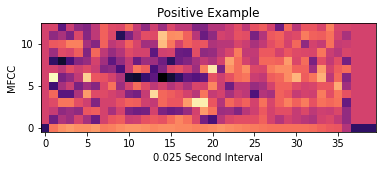
\includegraphics[width=0.5\textwidth]{figs/positive.png}}
    \caption{Positive Example}
    \label{fig:pos}
\end{figure}

\begin{figure}[htbp]
    \centerline{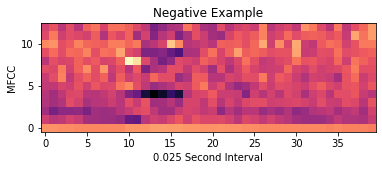
\includegraphics[width=0.5\textwidth]{figs/negative.png}}
    \caption{Negative Example}
    \label{fig:neg}
\end{figure}

\subsection{Convolutional neural net}

A standard image recognition convolutional neural net was chosen to label the "images"
created by the MFCC calculations \cite{hymel}.
This neural net consists of a series of convolution and max-pooling layers
followed by a few dense, flatten, and dropout layers.
As suggested by Google, the convolution layers utilize RelU activation,
and as suggested by Apple, the fully-connected output utilizes sigmoid activation
for an output in the $[0,1]$ range \cite{smallfoot} \cite{Efficient}.
Through experimentation, I was able to reduce the number of number of trainable parameters
by reducing the number of filters used in the convolution layers
without any adverse effect on model performance.
Figure \ref{fig:cnn} shows the Smithers model summary
and \ref{appendix:model} shows the code used to construct the model.

\begin{figure}[htbp]
    \centerline{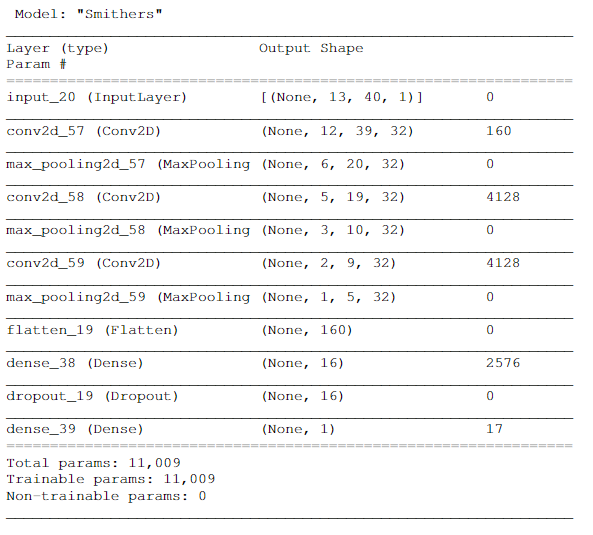
\includegraphics[width=0.5\textwidth]{figs/cnn.png}}
    \caption{Smithers CNN model summary}
    \label{fig:cnn}
\end{figure}


\subsection{Model Training, Validation, and Testing}
As mentioned in Section \ref{sec:dataset}, \textit{Dataset},
the 20,000-example dataset was split into 16,000 training examples,
2,000 validation examples, and 2,000 test examples.
Because Smithers is a binary classifier, the model was compiled
with a binary cross-entropy loss function.
Several different optimizers were tried with the best results 
produced by a stochastic gradient descent optimizer.

The model was fit with the training and validation data subsets.
The epoch count and batch size were adjusted experimentally
with the best results coming from 30 epochs and a 100-example batch size.
Figure \ref{fig:accuracy} and Figure \ref{fig:loss}
show the model training and validation accuracy and loss at each epoch.

\begin{figure}[htbp]
    \centerline{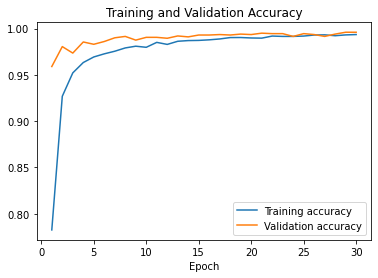
\includegraphics[width=0.5\textwidth]{figs/accuracy.png}}
    \caption{Model training and validation accuracy}
    \label{fig:accuracy}
\end{figure}
\begin{figure}[htbp]
    \centerline{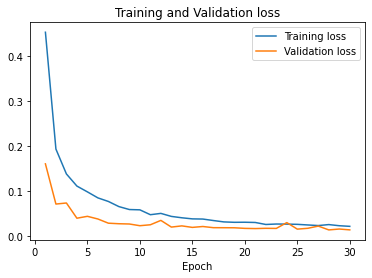
\includegraphics[width=0.5\textwidth]{figs/loss.png}}
    \caption{Model training and validation loss}
    \label{fig:loss}
\end{figure}

The model's test loss and accuracy were determined
by evaluating the model's performance on the 2,000-example test data subset
that was isolated from the model training and validation routines.
Calling the built-in Keras method Model.evaluate(),
the test lost was found to be $1.47\%$ and the test accuracy was found to be $99.6\%$
when evaluated with the test data subset.

\subsection{Model Deployment}
The model was saved as a TensorFlow Lite model for export to other devices.
TensorFlow Lite is a stripped-down version of the TensorFlow framework
used for "on-device inference" \cite{tensorflowlite}.
TensorFlow Lite is used on resource-constrained devices that down have the computing power
to run the full version of TensorFlow.
A TensorFlow Lite model is a single binary file that contains all the information needed
to run the model on any device.
This makes the model easily shareable - the Smithers TensorFlow Lite model, in fact, 
is only 46.5kB in size.

For real-time use of the Smithers model, a Python script was written
to continuously make predictions on one-second chunks of incoming audio.
This script uses the \textit{sounddevice} Python library to construct a
0.5-second long audio buffer and passes it to a callback function, twice per second.
This callback function builds a sliding window out of the 0.5-second audio buffer
to construct one-second long clip.
The MFCCs of this clip are calculated in the same way as in training
and the coefficients are evaluated by the TensorFlow Lite model.

Initially, this TensorFlow Lite model did not work at all.
It was eventually determined that the format of audio used in the training process
did not match the audio format of the real-time buffers.
This discrepancy was causing the MFCC calculations to differ between the two processes.
During the training process, the audio is stored as an array 16-bit integers.
For the real-time audio buffer, the sounddevice library stores the audio
as floating-point numbers in the $[-1,+1]$ range.
The fix turned out to be easy - the sounddevice InputStream method
accepts an optional parameter to specify the data type.
Appendix \ref{appendix:realtime} shows the sounddevice InputStream
and callback code used for the Smithers real-time implementation.


\section{Discussion of Results}

The Smithers model does an excellent job recognizing when I say "Hey Smithers".
I do not have any data on exactly \textit{how} well the model works
but, more often than not, Smithers correctly detects whenever I say the wake words.
I have not tested the model extensively, however, in a variety of environments
with a variety of different speakers.
It's likely the model won't work as well given different environmental conditions
and a speaker other than myself.
This model, however, serves well as a proof-of-concept and as a an excellent foundation
for further improvements.

The single greatest improvement made to this model was using a larger dataset.
Initially, only 400 positive and negative examples each were used.
Increasing this number to 10,000 examples each significantly improved model validation.
Additionally, changing the wake word from "Smithers" to "Hey Smithers" increased 
the model's accuracy.
I imagine the model can be further improved by training with more examples
from many different speakers and with a larger variety of environmental noise recordings.

Several optimizations were made to increase performance for resource-constrained devices.
The audio used in training and inference was downsampled from native the default 44.1kHz to 10kHz,
greatly decreasing the size of the data to be processed.
As suggested by Apple, the MFCCs were quantized from floating-point numbers to integers,
further decreasing the computational cost.
I was also able to reduce computational cost by reducing the number of filters
used in the convolutional neural net.
For Siri, Apple also quantized the CNN values between layers for even greater performance improvements.
This was not performed in this project but, according to Apple, quantizing the MFCCs and CNN values
decreased computational cost by over $75\%$ \cite{Efficient}.

I am interested in seeing how much meat I can strip off these bones -
how small can I make this model without severely sacrificing performance?
Sadeghi et al. have shown it is possible to correctly recognize words 
by using only the first 5 MFCCs \cite{optimalmfcc}.
I am interested in the performance impacts from reducing the number of MFCCs,
increasing the MFCC window length, lowering the sample rate of the audio streams,
and simplifying the CNN hyperparameters.

I found Python and the Keras and TensorFlow frameworks 
were incredibly intuitive for developing convolutional neural nets.
My prior efforts in building machine learning models all used MATLAB 
and Python has proven to be a much more enjoyable experience.
Best of all, Python is free and open source - this open access
makes it easy for anyone to get started exploring machine learning
without having to worry about paying for toolboxes or licenses.


\section{Conclusions}

\bibliographystyle{IEEEtran}
\bibliography{refs}

\newpage
\onecolumn
\appendix[Selected Code Excerpts]
\subsection{Data Synthesis Routine}\label{appendix:synthesis}
This routine synthesizes a data set from positive examples, negative examples, and noise clips.
This routine uses \textit{AudioSegment} from the \textit{pydub} Python library.

\begin{lstlisting}[language=Python]
def synthesize_sounds(num_sounds):  
    
    files_noise = file_list('.\\sounds\\raw\\noise')
    files_positive = file_list('.\\sounds\\raw\\positive')
    files_negative = file_list('.\\sounds\\raw\\negative')
    silence = AudioSegment.silent(duration=1000);

    i = 0
    while i < num_sounds :
        # select random background noise
        random_index = random.randrange(len(files_noise))
        raw_noise = AudioSegment.from_file(files_noise[random_index])
        # discard if background is shorter than 1000ms
        if(len(raw_noise) < 1000) : continue
        # randomly choose a 1000ms slice from the background
        slice_index = random.randrange(len(raw_noise) - 1000)
        raw_noise = raw_noise[slice_index:slice_index+1000]

        # select random positive 
        random_index = random.randrange(len(files_positive))
        raw_positive = AudioSegment.from_file(files_positive[random_index])
        # discard if raw_positive is greater than 1000ms
        if(len(raw_positive) > 1000) : continue

        # select random negative
        random_index = random.randrange(len(files_negative))
        raw_negative = AudioSegment.from_file(files_negative[random_index])
        # discard if raw_negative is greater than 1000ms
        if(len(raw_positive) > 1000): continue

        # randomly choose an insert point for the raw_positive
        insert_index = random.randrange(1000-len(raw_positive))
        positive_noisy = raw_noise.overlay(raw_positive, position=insert_index)
        positive_clean = silence.overlay(raw_positive, position=insert_index)

        #randomly choose an insert point for the raw_negative
        insert_index = random.randrange(1000-len(raw_negative) + 1)
        negative_noisy = raw_noise.overlay(raw_negative, position=insert_index)
        negative_clean = silence.overlay(raw_negative, position=insert_index)

        # export synthesized audio files
        positive_noisy.export('./sounds/synthesized/positive/positive_noisy_' + str(i) + '.wav', format='wav')
        positive_clean.export('./sounds/synthesized/positive/positive_clean_' + str(i) + '.wav', format='wav')
        negative_noisy.export('./sounds/synthesized/negative/negative_noisy_' + str(i) + '.wav', format='wav')
        negative_clean.export('./sounds/synthesized/negative/negative_clean_' + str(i) + '.wav', format='wav')
        
        i = i+1
    
synthesize_sounds(5000)
\end{lstlisting}

\subsection{MFCC Routine}\label{appendix:mfcc}
This routine calculates the MFCCs for each audio clip.

\begin{lstlisting}[language=Python]
def calc_mfcc(path):
    resample_rate = 10000
    # set to mono and downsample
    signal =  AudioSegment.from_wav(path).set_channels(1).set_frame_rate(resample_rate)
    signal = np.array(signal.get_array_of_samples())
    mfcc = python_speech_features.base.mfcc(signal, samplerate=resample_rate, winstep=0.025, numcep=13, winfunc=np.hanning)
    # quantize to 8-bit int
    mfcc = np.int8(mfcc)
    return mfcc.transpose()
\end{lstlisting}

\subsection{Keras Model Building}\label{appendix:model}
Keras was used to build the Smithers CNN model.

\begin{lstlisting}[language=Python]
shape = X_train[0].shape

M_input = Models.Input(shape=shape)
M = Layers.Conv2D(filters=32, kernel_size=(2,2), activation='relu')(M_input)
M = Layers.MaxPooling2D(pool_size=(2, 2), padding='same')(M)
M = Layers.Conv2D(32, (2, 2), activation='relu')(M)
M = Layers.MaxPooling2D(pool_size=(2, 2), padding='same')(M)
M = Layers.Conv2D(32, (2, 2), activation='relu')(M)
M = Layers.MaxPooling2D(pool_size=(2, 2), padding='same')(M)
M = Layers.Flatten()(M)
M = Layers.Dense(16, activation='relu')(M)
M = Layers.Dropout(0.5)(M)
M = Layers.Dense(1, activation='sigmoid')(M)
model = Models.Model(inputs=M_input, outputs=M, name="Smithers")
model.summary()   
\end{lstlisting}

\subsection{Real Time Prediction} \label{appendix:realtime}
\begin{lstlisting}[language=Python]
# sounddevice callback
def sd_callback(rec, frames, time, status):

    # remove unnecessary dimension
    rec = np.squeeze(rec)

    # sliding window
    window[:len(window)//2] = window[len(window)//2:]
    window[len(window)//2:] = rec

    # calculate mfccs
    mfcc = python_speech_features.base.mfcc(window, samplerate=resample_rate, winstep=0.025, numcep=13, winfunc=np.hanning)
    mfcc = np.int8(mfcc)
    mfcc = mfcc.transpose()

    # set up tensors
    in_tensor = np.float32(mfcc.reshape(1, mfcc.shape[0], mfcc.shape[1], 1))
    interpreter.set_tensor(input_details[0]['index'], in_tensor)
    interpreter.invoke()
    output = interpreter.get_tensor(output_details[0]['index'])
    prediction = output[0][0]

    # if "Hey Smithers" is detected
    if prediction > threshold:
        print('Hey Smithers detected!')

# set up sounddevice stream
with sd.InputStream(channels=1,
                    samplerate=resample_rate,
                    dtype='int16',
                    blocksize=int(resample_rate * buffer_length),
                    callback=sd_callback):
    while True:
        pass
\end{lstlisting}


\end{document}


